\documentclass{article}
\usepackage{graphicx}
\begin{document}
\hfill Alejandro Chavez

\hfill Lab 7 - Digital Logic

\hfill \today\\

\begin{center}\begin{large}Lab 7\end{large}\end{center}
Part 1
\begin{itemize}
	\item
		1-5)\\
    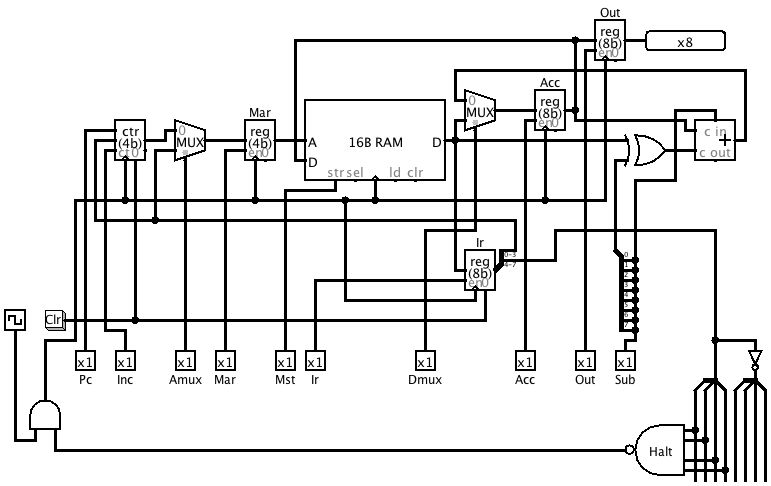
\includegraphics[scale=0.5]{lab7-1.png}
  \item
    6)\\
    The control code for this circuit has 10 bits.
\end{itemize}
Part 3
\begin{itemize}
  \item
    1)\\
    \begin{tabular}{cccccccccc|c}
    \multicolumn{10}{c|}{Control Code} & Action \\
    $Pc$ & $Inc$ & $Amux$ & $Mar$ & $Mst$ & $Ir$ & $Dmux$ & $Acc$ & $Out$ & $Sub$ & $f(src)\to dst$ \\ \hline
    $0$  & $1$   & $0$    & $1$   & $0$   & $0$  & $0$    & $0$   & $0$   & $0$   & $PC\to MAR;inc(PC)$ \\
    $0$  & $0$   & $0$    & $0$   & $0$   & $1$  & $0$    & $0$   & $0$   & $0$   & $Mem(MAR)\to IR$ \\
    \end{tabular}
  \item
    2)\\
    Out - 0101001110\\
    Hlt - 0101010000 (with the right contents at location 01)\\
  \item
    3)\\
    \begin{itemize}
      \item
        a)\\
        The initial value of the PC and IR are both 0.
      \item
        b)\\
        0101001110
      \item
        c)\\
        0x00 - 0x?? Anything can be here, as long as the most significant digit isn't F, since that will produce a halt signal in the machine. The contents at this address will be sent to the output pin.\\
        0x01 - 0xF? The most significant has to be F to produce a halt signal to the machine.
    \end{itemize}
  \item
    4)\\
    The instruction fetch control sequence works as expected. It takes three clock toggles to output the contents at 0x00 and halt.
\end{itemize}
Part 4
\begin{itemize}
  \item
    1)\\
    \begin{tabular}{cccccccccc|c}
    \multicolumn{10}{c|}{Control Code} & Action \\
    $Pc$ & $Inc$ & $Amux$ & $Mar$ & $Mst$ & $Ir$ & $Dmux$ & $Acc$ & $Out$ & $Sub$ & $f(src)\to dst$ \\ \hline
    $0$  & $1$   & $1$    & $1$   & $0$   & $1$  & $0$    & $0$   & $0$   & $0$   & $IR\to MAR$ \\
    $0$  & $0$   & $1$    & $1$   & $1$   & $0$  & $0$    & $0$   & $0$   & $0$   & $ACC\to Mem(MAR)$ \\
    \end{tabular}
    The instruction sequence works as expected.
  \item
    2)\\
    Once the halt instruction is loaded into the IR, game over; you can't toggle the clock anymore.
\end{itemize}
\end{document}
